% !TeX root = ../main.tex

\chapter{区块链技术}

\section{区块链系统简介}

区块链技术旨在不可信的开放网络中,维护一个安全可信、不可篡改的公共账本,并以此为基础构建电子 交易、访问控制等应用系统.根据新节点的加入是否需要授权认证,区块链系统可以分为许可链和非许可链两 大类.非许可链通常也称为公有链,不限制节点的加入或退出,任何节点可以访问链上数据、发布交易、以及 参与链上数据的记录,甚至可以尝试发布不合法消息,攻击网络中的其他节点.许可链指区块链网络中节点 的加入网络、记录账本等操作需要经过特定的授权许可与认证.许可链系统又可以根据系统参与方的数量分 为联盟链与私有链,其中联盟链由多方组织加入同一区块链网络中,共同维护区块链账本,记录并执行链上合 约,多方组织可以通过一致的账本建立起联盟成员之间的信任.而私有链通常由一个参与方负责创建和维护, 主要用于记录和管理内部数据,增强数据的安全性、可追溯性. 

本文对比许可链和非许可链两类区块链系统在准入限制、参与方数量、采用的共识算法、应用场景等方面的区别,并总结如表\ref{tab:classification} 所示. 

\begin{table}[htb]
  \centering
  \begin{minipage}[t]{1\linewidth} % 如果想在表格中使用脚注,minipage是个不错的办法
  \caption[模板文件]{区块链系统分类}
  \label{tab:classification}
    \begin{tabularx}{\linewidth}{lXX}
      \toprule[1.5pt]
      {\heiti 名称} & {\heiti 非许可链} & {\heiti 许可链} \\\midrule[1pt]
		准入限制  & 无准入限制,任意节点可以随时加入或者退出 & 有准入限制,准入限制由整个联盟的节点商议后制定 \\
		参与方数量  & 较多 & 较少 \\  
		共识算法  & POW, POS等共识算法 & BFT类分布式共识算法 \\  
		区块链性能  & 较低 & 较少 \\  
		应用场景	 & 密码货币交易系统 & 公司间合同,公司内事务管理 \\  
		典型应用  & Bitcoin, Ethereum & HyperLedger, Coco \\
      \bottomrule[1.5pt]
    \end{tabularx}
  \end{minipage}
\end{table}

\section{密码学基础}

区块链系统中引入大量的密码学技术提供安全性、可信性等密码学性质,并以此作为区块链价值的底层保障。目前主要有哈希算法、非对称加密体制、电子签名、布尔集合、密码累加器、同态加密、零知识证明、安全多方计算等密码学技术用于区块链系统。本章主要介绍广泛应用的哈希算法,非对称加密,电子签名和布尔过滤器。

\subsection{哈希函数}

哈希函数,通常也称散列函数,是一种将任意长度的输入转换为固定长度的输出的函数。哈希函数的表示形式为:
$$h=H(m)$$
其中,m为任意长度消息,H为哈希函数,h为固定长度的哈希值,通常也称为消息摘要。

哈希函数具有如下特性:
\begin{enumerate}
\item 单向性:从输入计算输出很简单,但在不知道输入的情况下,通过输出计算出输入是计算上不可行的;
\item 输出的随机性:即算法输出的每一位数据在统计学意义上都符合随机分布;
\item 雪崩效应:对输入的任何一点修改,都会导致输出的大量变化;
\item 抗碰撞性:找到两个具有相同的输出的不同输入,是计算上不可行的。
\end{enumerate}

正是由于上述重要特性,哈希算法被广泛应用于消息认证码、随机数产生、错误校正与检测等领域,而在区块链系统中,哈希算法主要用于检查数据是否被篡改,提供工作量证明,构造存在性证明这几个用途。传统互联网中,哈希算法常用于数据的完整性验证。为了验证互联网中的文件在传输过程中是否被篡改,通常采用存储验证文件哈希值的方式,利用了哈希函数的雪崩效应和抗碰撞性,一旦数据被篡改,最终的哈希值一定与之前存储的哈希值不同。而在区块链系统中,由于交易数据不断增长,账户状态不断变化,如果采用全部数据求哈希值的方法,则每次改变都需要重新计算哈希值,计算复杂度不可接受。因此,在区块链系统中,数据根据时间顺序组织成了若干个区块,一定时间内新发生的事务数据存储在一个新区块里,每一个区块都包含了上一个区块的哈希值。这样的数据组织方式如同区块形成的链状结构,因而称为区块链。具体组织结构如图\ref{fig:hashchain}所示。


\begin{figure}
\centering	
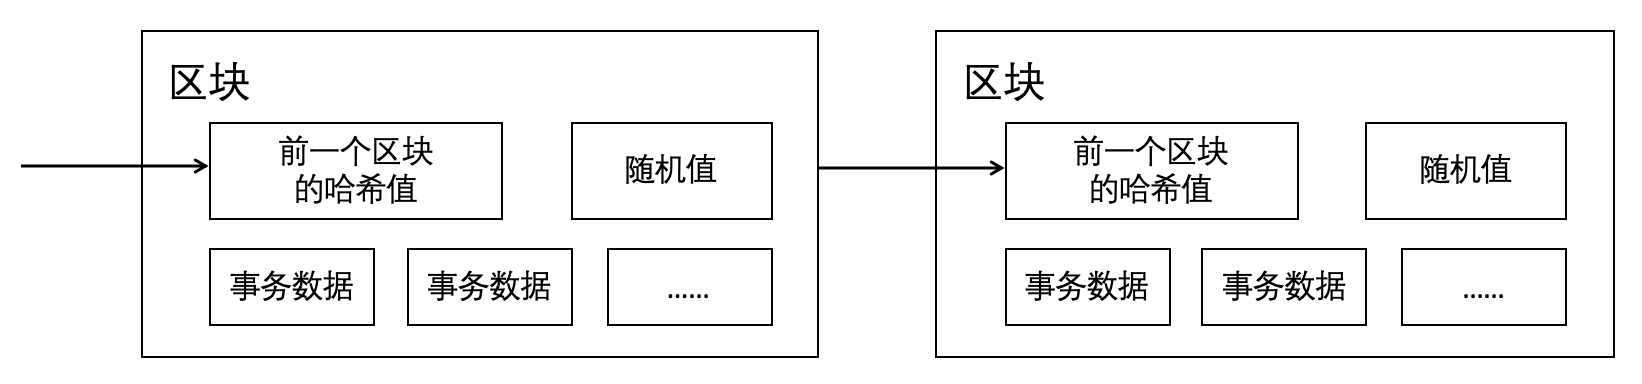
\includegraphics [width=400pt,height=100pt]{figures/hashchain.png}
\caption{区块链数据结构}
\label{fig:hashchain}
\end{figure}

如果区块链中任意区块里的数据被篡改,那么该区块的哈希值与后一区块记录的哈希值不相等。由哈希函数的雪崩效应可知,区块链上的任何历史数据改动都能被检测。因此,节点只需要存储最新区块的哈希值,即可通过计算检验历史上所有区块中的数据是否被篡改。

\begin{figure}
\centering	
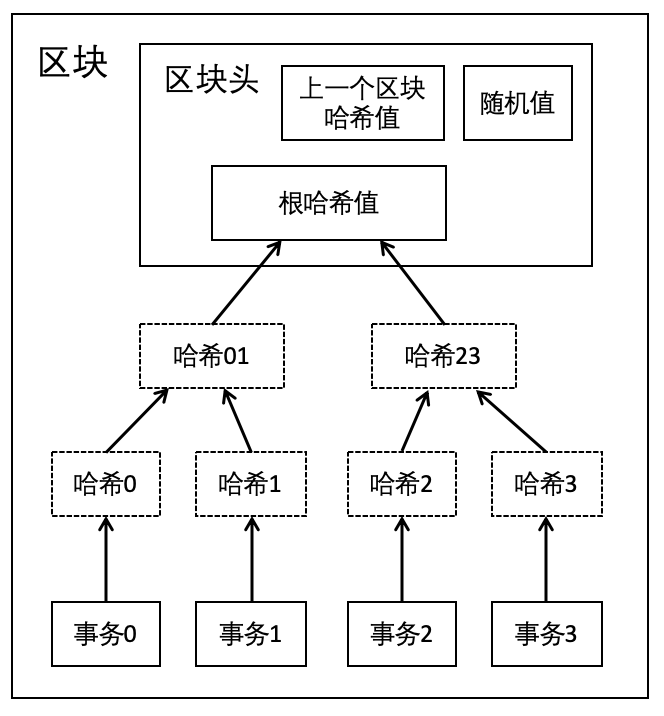
\includegraphics [width=150pt,height=180pt]{figures/merkle-tree.png}
\caption{默克尔树数据结构}
\label{fig:merkle-tree}
\end{figure}

而在每个区块中,哈希函数用于构建默克尔树,即哈希二叉树。如图\ref{fig:merkle-tree}所示,所有事务的哈希值通过二叉树结构进行哈希计算,最终计算得到根哈希值。该数据结构保证,任意事务数据的修改,都会影响到根哈希值。因此区块头中只需要存储根哈希值,就可以验证该区块中所有事务是否被篡改。


\begin{figure}
\centering	
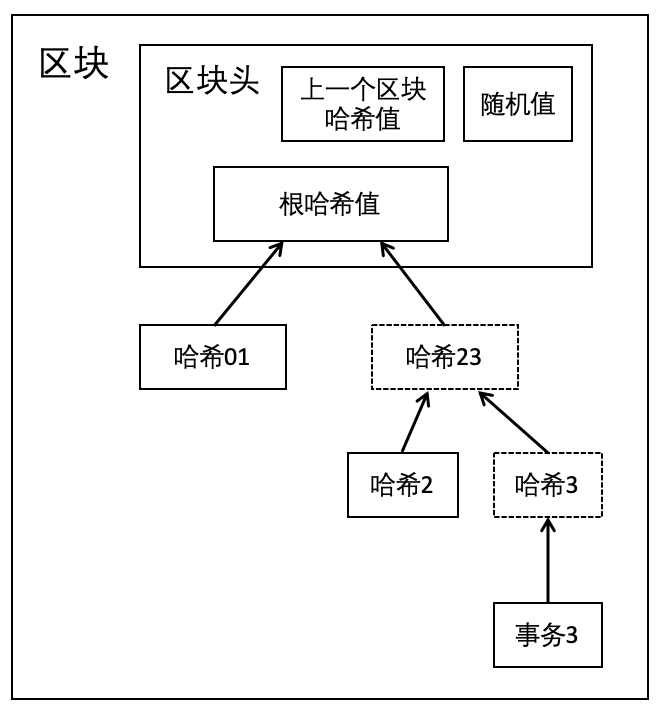
\includegraphics [width=150pt,height=180pt]{figures/merkle-proof.png}
\caption{交易存在性证明}
\label{fig:merkle-proof}
\end{figure}

当用户需要通过根哈希值验证某事务是否在某区块中时,不需要验证该区块中所有事务数据,只需要由存储所有数据的节点提供该事务到根哈希值的路径上所有相关数据。如图\ref{fig:merkle-proof}所示,当用户希望验证事务3是否存储在区块中,只需要验证“事务3”,“哈希2”,“哈希01”这几个数据是否能通过哈希函数得到根哈希值。由哈希函数的抗碰撞性可以保证,证明节点不能提供虚假数据计算出同样的根哈希值。

\subsection{非对称密码体制和电子签名}

密码体制主要分为对称密码体制和非对称密码体制。简单来说,对称密码体制指加密算法中使用的加密密钥和解密算法中使用的解密密钥是相同的密钥,或者解密密钥能通过加密密钥计算得到。而非对称密码体制中,这两者不同,并且解密密钥不能通过加密密钥计算得到。

\begin{figure}
\centering	
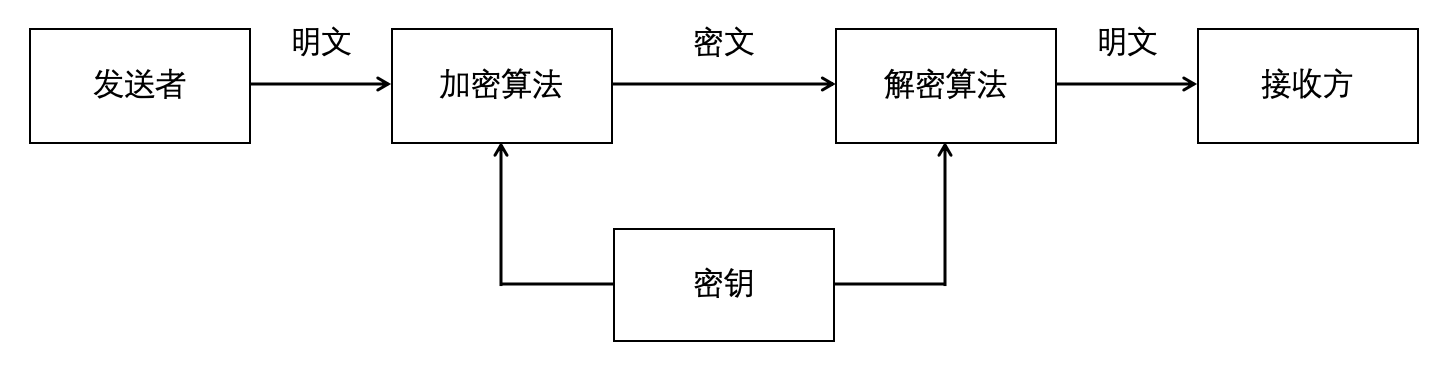
\includegraphics [width=400pt,height=100pt]{figures/sym-crypto.png}
\caption{对称密码体制的基本模型}
\label{fig:sym-crypto}
\end{figure}

如图\ref{fig:sym-crypto}所示,对称密码体制中,发送者先使用密钥和加密算法将明文加密为密文,然后传输密文给接收方,接收方使用解密算法和相同的密钥将密文解密回原始的明文。因为加密和解密算法使用的密钥需要相同,消息发送方和接收方必须在密文传输前通过安全信道进行密钥传输。因此对称密码体制面临密钥分配问题,目前主要通过通信双方直接进行密钥传输或者密钥分配中心进行密钥分发进行。然而实际的传输信道安全性并不理想,密钥在传输过程中被暴露的风险很大,增加了系统的脆弱性。另一方面,在有多个用户的网络中,任何两个用户之间都需要共享加密密钥。当网络中用户$n$很大时,需要管理的密钥数目为$C_n^2$,复杂度近似O($n^2$)。当有一个新用户加入时,需要产生$n$个秘密的密钥,并秘密分发给$n$个用户。对称密码体制中使用的加密算法主要采用扩散和混淆两种基本方法,可以抵抗密码分析技术对密文进行统计分析。扩散指让明文中的每一位尽可能多影响密文中的若干位,以及让密文中的每一位受到明文中尽可能多位的影响,这样可以隐蔽明文的统计特性。字符到字符的映射,通常包含单字符置换和多字符置换。混淆指混淆密文与密钥之间的统计关系,使得对手即使获取了关于密文的一些统计特性,也无法推测密钥。通常使用复杂的非线性代替变换可以达到比较好的混淆效果。

\begin{figure}
\centering	
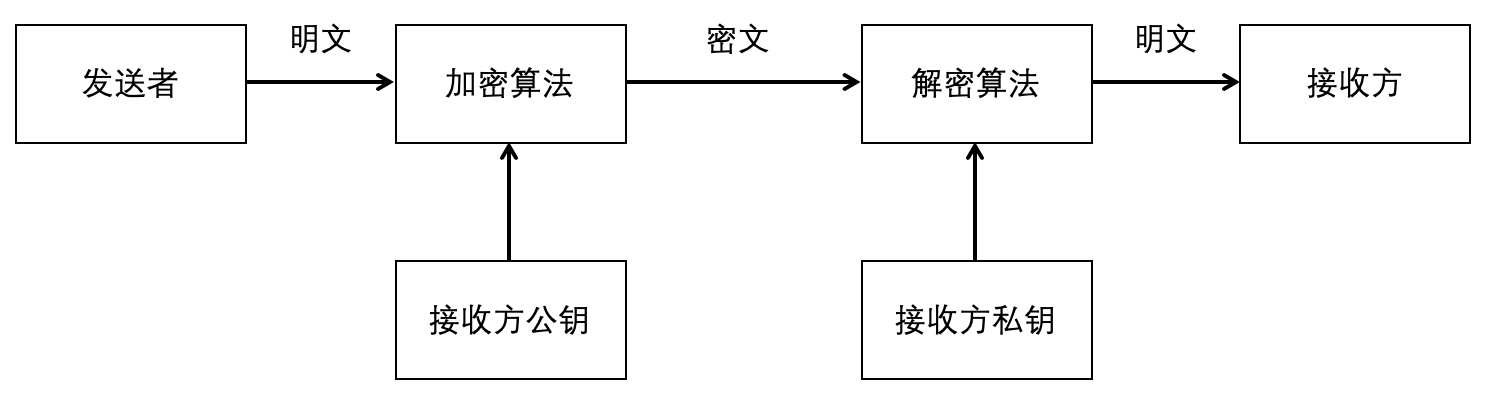
\includegraphics [width=400pt,height=115pt]{figures/asym-crypto.png}
\caption{非对称密码体制的基本模型}
\label{fig:asym-crypto}
\end{figure}

1976年,W.Diffie和M.Hellman在IEEE Trans.on Information刊物上发表了“ New Direction in Cryptography”文章,提出了“非对称密码体制“的概念,开创了密码学研究的新方向。如图\ref{fig:asym-crypto}所示,非对称密码体制中,密钥分为成对的加密密钥和解密密钥,其中加密密钥公开,解密密钥保密。公开的密钥可以作为用户的个人身份,由公开的加密密钥无法推导相应的解密密钥。因此即使将加密密钥公开也不会暴露解密密钥,不会损害密码的安全。因此,通信双方可以通过不安全的信道交换公钥,然后用对方的公钥对消息进行加密并传输,达到在不安全的信道上保密传输的效果。解决了对称密码体制中需要安全信道的问题,同时在密钥管理上也极大降低了网络中需要管理的密钥数量,从对称密码体制的$C_n^2$降低到$n$。对称密码体制与非对称密码体制在密钥分发、密钥管理等方面的区别主要如表\ref{tab:sym-asym}所示。

\begin{table}[htb]
  \centering
  \begin{minipage}[t]{1\linewidth}
  \caption{对称密码体制与非对称密码体制的区别}
  \label{tab:sym-asym}
    \begin{tabularx}{\linewidth}{lXX}
      \toprule[1.5pt]
      {\heiti 功能} & {\heiti 对称密码体制} & {\heiti 非对称密码体制} \\\midrule[1pt]
		密钥分发  & 需要事先进行安全的密钥分发 & 不需要事先进行安全的密钥分发,公钥可以在不安全的信道上传输 \\
		密钥管理  & 每个用户需要保存n个不同密钥用于与其他n个用户通信。当有新用户加入时,每个用户都需要和新用户共享一个新密钥,整个系统中需要存储O($n^2$)个密钥 & 每个用户只需要存储自己的公钥和私钥,整个系统中只需要存储O(n)个密钥 \\
		电子签名  & 不支持电子签名功能 & 支持电子签名功能 \\  
		性能  & 加密算法和解密算法简单,加解密速度较快 & 加密算法和解密算法需要进行复杂的数学运算,速度较慢 \\  
		安全性  & 安全性来源于混淆和置换 & 安全性通常基于数学难问题,部分假设未证明 \\ 
      \bottomrule[1.5pt]
    \end{tabularx}
  \end{minipage}
\end{table}

数字签名,通常也称为电子签名,指通过数据处理的方式对数字消息进行签名。同样具有手写签名的两大特性:可验证性和防伪造性。具体来说,数字签名需要具备以下特性:

\begin{enumerate}
 \item 任何人可以验证数字签名是否由消息的发送方生成。
 \item 任何人不能伪造发送方的数字签名,这也意味着发送方不能抵赖自己生成的数字签名。
 \item 任何人可以验证数字签名是否匹配发送的消息,因此可以验证消息从发送到接受过程中是否被篡改。对整个消息生成数字签名过于复杂,因此通常先对消息计算哈希值,然后生成哈希值的数字签名用于验证。
\end{enumerate}

某种意义上,我们可以认为数字签名的过程是一种加密,而对签名还原到原消息,然后进行验证是一种解密。但与非对称公钥体系中的公钥加密,私钥解密恰好相反,通过私钥计算签名,然通过公钥进行验证。由于公钥公开,因此所有人可以知道该公钥的持有者。而只有该用户拥有对应的私钥,才能生成正确的数字签名。

在区块链领域,每个用户都可以通过特定算法独立生成任意多账户,即公私钥对。当用户发起事务时,需要用私钥生成事务数据的电子签名。当该事务涉及其他用户时,使用特定用户公钥生成的地址。

\subsection{布尔过滤器}

为了验证某数据是否存在集合中,传统算法主要有遍历查找,二分查找,索引查找等,这些算法的时间消耗都会随着集合数量的增加而增加。为了解决这一问题,布尔过滤器利用哈希算法的输出长度固定性和随机性,利用固定长度的数组存储集合,对元素进行哈希变换,然后根据输出找到对应下标并在数组中记录或查询。为了解决不同输入映射到同一下标的问题,通常采用多个哈希函数共同确认。布尔过滤器具有很好的空间和时间效率,被用来检测一个元素是不是集合中的一个成员。在以太坊项目中,布尔过滤器被用于检测交易是否在给定区块中,便于用户快速检索特定交易的存储位置。和布尔过滤器类似,密码累加器也用于高效验证数据的存在性,后者还可以提供高效安全的存在性证明。在零币项目中,密码累加器用于存储用户加入的未花费代币的对应编码,当用户使用时,其他用户可以高效验证花费的代币是否存在。

\section{共识协议}

\subsection{传统分布式共识协议}
\label{subsec:traditional-consensus}

PAXOS

RAFT

PBFT

\subsection{工作量证明共识协议}
\label{subsec:work-proof}

在区块链领域,尤其在公有链网络中,节点可以自由加入或退出网络,因此无法采用基于身份投票的方式。传统的分布式共识算法无法使用。因此在公有链领域广泛使用比特币系统提出的工作量证明共识算法及其变形。

首先我们介绍比特币系统提出的工作量证明算法,工作量证明最早用于抵抗针对邮件服务器的拒绝服务攻击以及防止垃圾邮件的发送。

为了解决比特币系统的性能瓶颈,以太坊项目提出了GHOST协议,该协议将最长链共识原则改为最大子树共识原则。

而以太坊提出的最大子树共识只利用了分叉块的工作量,为了进一步提升系统性能,conflux协议在此基础上进一步利用了分叉块中未冲突的交易。


